\documentclass[12pt]{article}

\usepackage[T3]{fontenc}
\usepackage[utf8]{inputenc}
\usepackage[russian]{babel}

\usepackage{mhchem}
\usepackage{amssymb, amsmath}

\usepackage{tikz}
\usetikzlibrary{shapes.geometric, arrows, positioning, decorations.markings}
\usetikzlibrary{fit}
\usepackage{microtype}
\usepackage{framed}
\usetikzlibrary{decorations.pathmorphing,calc,backgrounds}

\usepackage{animate}

\usepackage{fixltx2e}
\usepackage{hyperref}

%\usetheme{Berkeley}
%\usetheme{Madrid} -- неплохо
%\usetheme{CambridgeUS}
%\usetheme{Singapore}
\usetheme{Warsaw}

\pdfmapfile{+sansmathaccent.map}

\title{Исследование бифуркаций в трехатомных гидридах методом классических траекторий}

\author{\small 
Финенко Артем \\[1ex] 
Научный руководитель: Петров С.В.}

\institute[MSU] % (optional, but mostly needed)
{
  МГУ им. М.В.Ломоносова \\
  Химический факультет
}

\date{23/12/2016}

\pgfdeclareimage[height=0.5cm]{university-logo}{../pictures/logo.jpg}
\logo{\pgfuseimage{university-logo}}

\newcommand\Fontvi{\fontsize{6}{7.2}\selectfont}

\beamertemplatenavigationsymbolsempty

\setbeamerfont{page number in head/foot}{size=\large}
\setbeamertemplate{footline}[frame number]
\setbeamertemplate{frametitle}[default][center]

% change font
\usefonttheme[onlymath]{serif}

% custom block environment
\newenvironment<>{varblock}[2][.9\textwidth]{%
  \setlength{\textwidth}{#1}
  \begin{actionenv}#3%
    \def\insertblocktitle{#2}%
    \par%
    \usebeamertemplate{block begin}}
  {\par%
    \usebeamertemplate{block end}%
  \end{actionenv}}

\tikzstyle{lagrange} = [rectangle, rounded corners, minimum width = 3cm, minimum height = 1cm, text centered, text width = 5cm, draw = black, fill=DarkOrchid!40]

\tikzstyle{equations} = [rectangle, rounded corners, text centered, draw = black, fill=green!30]

\tikzstyle{hamilton} = [rectangle, rounded corners, minimum width = 3cm, minimum height = 1cm, text centered, text width = 5 cm, draw = black, fill = Goldenrod!50]

\tikzstyle{result} = [rectangle, rounded corners, text centered, draw = black, fill = blue!30]

\tikzstyle{arrow} = [thick, ->, >=stealth]

\tikzstyle{vecArrow} = [thick, decoration={markings,mark=at position
   1 with {\arrow[semithick]{open triangle 60}}},
   double distance=1.4pt, shorten >= 5.5pt,
   preaction = {decorate},
   postaction = {draw,line width=1.4pt, white,shorten >= 4.5pt}]

\usepackage{caption}
\usepackage{subcaption}

% SKIPS
% "\," -- very small skip

\begin{document}

\begin{titlepage}
\centering
\textbf{\large Московский государственный университет имени М.В.\,Ломоносова\\
\vspace*{0.1cm} Химический факультет\\
\vspace*{0.1cm}
\noindent\makebox[\linewidth]{\rule{\paperwidth}{0.4pt}}
\vspace*{0.1cm}
 Кафедра физической химии\\
\vspace*{0.1cm} Лаборатория строения и квантовой механики молекул \\}
\vspace*{2cm}

\begin{center}

\includegraphics[width=0.3\textwidth]{../pictures/logo.jpg}
\end{center}

\vspace*{2cm}
\Large \textbf{Исследование бифуркаций в трехатомных гидридах методом классических траекторий.}
\vspace*{2cm}

\begin{flushright}
\large Курсовая работа студента 411 группы\\
Финенко А.А.\\
\vspace{1cm}
Научный руководитель:\\
к.ф.-м.н., с.н.с. Петров С.В.
\end{flushright}
\vfill
\large\textbf{Москва\\ 2016}
\end{titlepage}


\tableofcontents

\newpage

\section{Введение}

\section{Схема получения полного колебательно-вращательного гамильтониана}
\subsection{Переход в систему отсчета, связанную с центром масс}

\hspace{0.35cm} Рассмотрим систему $n$ материальных точек. Обозначим их массы через $m_i$, их радиус-векторы в лабораторной системе координат через $\vec{r}_i$, в подвижной системе координат -- через $\vec{R}_i$ ($i = 1 \dots n$). Разделим движение системы на движение центра масс и движение вокруг центра масс:
\vspace*{-0.1cm}
\begin{gather}
\left\{
\begin{aligned}
\vec{r}_1 &= \vec{r} + \vec{r}_1^{\ \prime}, \\
&\cdots \\
\vec{r}_n &= \vec{r} + \vec{r}_n^{\ \prime},
\end{aligned}
\right. \notag
\end{gather}

\hspace*{-0.75cm} где $\vec{r}$ -- радиус-вектор центра масс в лабораторной системе координат и $\vec{r}_i^{\ \prime}$ -- радиус-векторы рассматриваемых точек в системе отсчёта, связанной с центром масс.

Кинетическая энергия $T$ системы принимает вид: 
\vspace*{-0.1cm}
\begin{gather}
T = \frac{1}{2} \sum_{i=1}^{n} m_i \dot{\vec{r}}_i^{\ 2} = \frac{1}{2} \sum_{i=1}^{n} m_i (\dot{\vec{r}} + \dot{\vec{r}}_i^{\ \prime})^2  = \frac{1}{2} M \dot{r}^2 + \frac{1}{2} \sum_{i=1}^{n} m_i ( \dot{r}_i^\prime)^2 + \dot{\vec{r}} \sum_{i=1}^{n} m_i \dot{\vec{r}}_i^{\ \prime}, \notag
\end{gather}

\hspace*{-0.75cm} где $M = \sum_{i=1}^{n} m_i$.

Заметим, что последняя сумма является производной следующей суммы, которая равна нулю: 
\vspace*{-0.1cm}
\begin{gather}
\sum_{i=1}^{n} m_i \dot{\vec{r}}_i^{\ \prime} = \frac{d}{dt} \sum_{i=1}^{n} m_i \vec{r}_i^{\ \prime} = 0. \notag
\end{gather}

Итак, мы перешли в систему координат, связанную с центром масс, и отделили энергию движения центра масс:
\vspace*{-0.1cm}
\begin{gather}
T = \frac{1}{2} M \dot{r}^2 + \frac{1}{2} \sum_{i=1}^{n} m_i( \dot{r}_i^\prime)^2. \notag
\end{gather}

Забудем про слагаемое, отвечающее центру масс; откинем штрихи, чтобы упростить запись.

\subsection{Переход в подвижную систему отсчета}

Переход от лабораторной системы отсчета к подвижной системе может быть осуществлен при помощи трех последовательных поворотов на углы Эйлера $\varphi$, $\theta$ и $\psi$. 

\begin{figure}
  \centering
	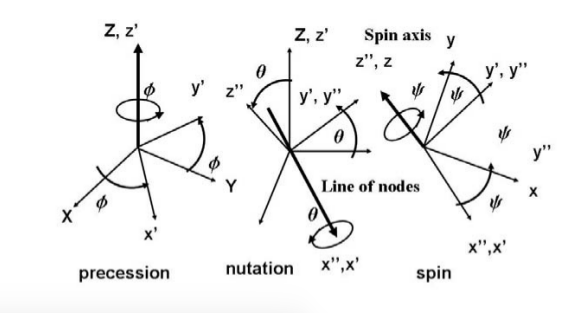
\includegraphics[width=0.7\textwidth]{../pictures/EulerAngles.jpg}
	\caption{Углы Эйлера}
	\label{fig:EulerAngles}
\end{figure}

Первое вращение происходит вокруг оси $z$ на угол $\varphi$. Оно переводит лабораторную систему $x, y, z$ в систему $x^\prime$, $y^\prime$, $z^\prime$. Угол $\varphi$ называется углом прецессии.
\begin{gather}
\begin{pmatrix}
x^\prime \\
y^\prime \\
z^\prime
\end{pmatrix} = 
\begin{pmatrix}
\cos \varphi & \sin \varphi & 0 \\
- sin \varphi & \cos \varphi & 0 \\
0 & 0 & 1
\end{pmatrix}
\begin{pmatrix}
x \\
y \\
z
\end{pmatrix} =
\bbS_\varphi
\begin{pmatrix}
x \\
y \\
z
\end{pmatrix} \notag
\end{gather}

Оси  $x^\prime$, $y^\prime$ лежат в плоскости $x$, $y$. Затем происходит поворот вокруг оси $x^\prime$ на угол $\theta$, переводящий систему $x^\prime$, $y^\prime$, $z^\prime$ в систему $x^{\dpr}$, $y^{\dpr}$, $z^{\dpr}$. Ось $x^{\dpr}$ совпадает с осью $x^{\prime}$. Ось этого поворота называется линией узлов. Угол $\theta$ называется углом нутации.

\begin{gather}
\begin{pmatrix}
x^{\dpr} \\
y^{\dpr} \\
z^{\dpr} 
\end{pmatrix} = 
\begin{pmatrix}
1 & 0 & 0 \\
0 & \cos \theta & \sin \theta \\
0 & - sin \theta & \cos \theta
\end{pmatrix}
\begin{pmatrix}
x^\prime \\
y^\prime \\
z^\prime
\end{pmatrix} = 
\bbS_\theta
\begin{pmatrix}
x^\prime \\
y^\prime \\
z^\prime
\end{pmatrix} \notag
\end{gather}   

И наконец, вращение вокруг оси $z^{\dpr}$ на угол $\psi$ переводит систему $x^{\dpr}$, $y^{\dpr}$, $z^{\dpr}$ в систему $x$, $y$, $z$. Угол $\psi$ называется углом собственного вращения.

\begin{gather}
\begin{pmatrix}
X \\
Y \\
Z
\end{pmatrix} =
\begin{pmatrix}
\cos \psi & \sin \psi & 0 \\
- \sin \psi & \cos \psi & 0 \\
0 & 0 & 1
\end{pmatrix}
\begin{pmatrix}
x^{\dpr} \\
y^{\dpr} \\
z^{\dpr}
\end{pmatrix} = 
\bbS_\psi 
\begin{pmatrix}
x^{\dpr} \\
y^{\dpr} \\
z^{\dpr}
\end{pmatrix} \notag
\end{gather}

Суммарное вращение представляет собой последовательное применение описанных поворотов и имеет следующую матрицу: 
\begin{gather}
\begin{pmatrix}
X \\
Y \\
Z
\end{pmatrix} = 
\bbS 
\begin{pmatrix}
x \\
y \\
z
\end{pmatrix} \notag \\
\bbS = \bbS_\psi \bbS_\theta \bbS_\varphi = 
\begin{pmatrix}
\cos \psi \cos \varphi - \cos \theta \sin \varphi \sin \psi & \cos \psi \sin \varphi + \cos \theta \cos \varphi \sin \psi & \sin \theta \sin \psi \\
- \sin \psi \cos \varphi - \cos \theta \sin \varphi \cos \psi & - \sin \psi \sin \varphi + \cos \theta \cos \varphi \cos \psi & \sin \theta \cos \psi \\
\sin \psi \sin \theta & - \cos \varphi \sin \theta & \cos \theta 
\end{pmatrix} \notag
\end{gather}

Проектируя вектор угловой скорости $\Omega$ на базис, образованный Эйлеровыми угловыми скоростями $\dot{\varphi}$, $\dot{\theta}$, $\dot{\psi}$, получаем соотношение, известное как кинематическое уравнение Эйлера:

\begin{gather}
\begin{pmatrix}
\Omega_X \\
\Omega_Y \\
\Omega_Z
\end{pmatrix} =
\begin{pmatrix}
\sin \theta \sin \psi & \cos \psi & 0 \\
\sin \theta \cos \psi & - \sin \psi & 0 \\
\cos \theta & 0 & 1
\end{pmatrix}
\begin{pmatrix}
\dot{\varphi} \\
\dot{\theta} \\
\dot{\psi}
\end{pmatrix} \notag
\end{gather}

\begin{figure}
  \centering
	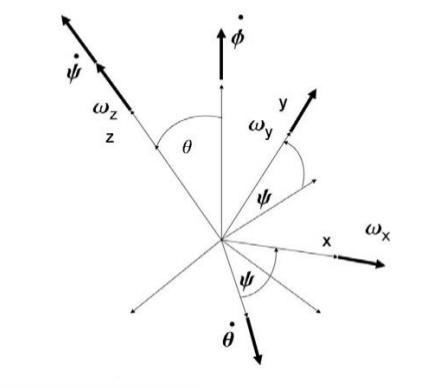
\includegraphics[width=0.5\textwidth]{../pictures/AngularVelocities.jpg}
	\caption{Угловые скорости}
	\label{fig:AngularVelocities}
\end{figure}

ПОПРАВИТЬ НА КАРТИНКЕ МАЛЕНЬКИЕ БУКВЫ НА БОЛЬШИЕ

Я НЕ ЗНАЮ КАК СВЯЗАТЬ НАПИСАННОЕ НИЖЕ С ТЕМ, ЧТО ДОПИСАНО СЕЙЧАС

Перейдём в подвижную систему координат при помощи ортогональной матрицы $\bbS$:
\vspace*{-0.1cm}
\begin{gather}
\vec{r}_i = \bbS \vec{R}_i, \quad i = 1 \dots n. \notag
\end{gather}

Введем матрицу $\bbA$ следующим образом: $\bbA = \dot{\bbS} \bbS^{-1}$. Покажем, что она является кососимметрической матрицей; для этого продифференцируем единичную матрицу:
\vspace*{-0.1cm}
\begin{gather}
\frac{d}{dt} \bbE = \frac{d}{dt} \left( \bbS \bbS^{-1}\right) = \dot{\bbS} \bbS^{-1} + \bbS \dot{\bbS}^{-1} = 0. \notag
\end{gather}

Заметим, что первое слагаемое и есть матрица $\bbA$, а второе -- транспонированная матрица $\bbA$ (т.к. $\bbS^\top = \bbS^{-1}$ в силу ортогональности). Следовательно,
\vspace*{-0.1cm}
\begin{gather}
\bbA + \bbA^\top = 0, \notag
\end{gather}

\hspace*{-0.75cm} т.е. по определению матрица $\bbA$ является кососимметрической.

Так как размерность пространства кососимметрических матриц равна 3, то существует естественный изоморфизм, позволяющий сопоставить каждой кососимметрической матрице единственный псевдовектор:
\vspace*{-0.1cm}
\begin{gather}
\bbA = 
\begin{pmatrix}
0 & -\omega_3 & \omega_2 \\
\omega_3 & 0 & -\omega_1 \\
-\omega_2 & \omega_1 & 0
\end{pmatrix}
\quad
\longleftrightarrow
\quad
\vec{\omega} = 
\begin{pmatrix}
\omega_1 \\
\omega_2 \\
\omega_3
\end{pmatrix}
,
\notag
\end{gather}

\hspace*{-0.75cm} причем для любого вектора $\vec{x} \in \mathbf{R}^3$ имеем $\bbA \vec{x} = [ \vec{\omega} \times \vec{x} ]$, где $\vec{\omega}$ -- вектор угловой скорости в лабораторной системе координат.

Получим выражение для квадратов скоростей рассматриваемых точек в лабораторной системе координат через координаты и скорости в подвижной системе координат:
\vspace*{-0.1cm}
\begin{gather}
\dot{\vec{r}}_i = \bbS \dot{\vec{R}}_i + \dot{\bbS} \vec{R}_i = \dot{\bbS} \bbS^{-1} \vec{r}_i + \bbS \dot{\vec{R}}_i  = \bbA \vec{r}_i + \bbS \dot{\vec{R}}_i = [ \vec{\omega} \times \vec{r}_i ] + \bbS \dot{\vec{R}}_i = [\bbS \vec{\Omega} \times \bbS \vec{R}_i ] + \bbS \dot{\vec{R}}_i = \notag \\
= \bbS \left( [\vec{\Omega} \times \vec{R}_i ] + \dot{\vec{R}}_i \right)  \notag , \\
\dot{r}_i^2 = \dot{\vec{r}}_i^{\ \top} \dot{\vec{r}}_i = \left( \dot{\vec{R}}_i + [ \vec{\Omega} \times \vec{R}_i] \right)^\top \bbS^\top \bbS \left( \dot{\vec{R}}_i + [ \vec{\Omega} \times \vec{R}_i ] \right) = \dot{R}_i^2 + 2 \dot{\vec{R}}_i \ [ \vec{\Omega} \times \vec{R}_i] + [ \vec{\Omega} \times \vec{R}_i ]^2 \notag ,
\end{gather}

\hspace*{-0.75cm} где $\vec{\Omega}$ -- вектор угловой скорости в подвижной системе координат.

Рассмотрим последнее слагаемое как смешанное произведение и применим правило Лагранжа:
\vspace*{-0.1cm}
\begin{gather}
([\vec{\Omega} \times \vec{R}_i] , [\vec{\Omega} \times \vec{R}_i]) = \vec{\Omega}^\top [ \vec{R}_i \times [ \vec{\Omega} \times \vec{R}_i ]] = \vec{\Omega}^\top \left( \vec{\Omega} (\vec{R}_i, \vec{R}_i ) - \vec{R}_i (\vec{R}_i, \vec{\Omega} ) \right)
\notag .
\end{gather}

Итак, с учётом выполненных преобразований имеем:
\vspace*{-0.1cm}
\begin{gather}
T = \frac{1}{2} \sum_{i=1}^{n} m_i \dot{r}_i^2 = \frac{1}{2} \sum_{i=1}^{n} m_i \dot{R}_i^2 + \vec{\Omega} ^\top \sum_{i=1}^{n} m_i[ \vec{R}_i \times \dot{\vec{R}}_i ] + \frac{1}{2} \vec{\Omega}^\top \sum_{i=1}^{n} m_i \left( \vec{\Omega} (\vec{R}_i, \vec{R}_i ) - \vec{R}_i (\vec{R}_i, \vec{\Omega} ) \right) = 
\notag \\
= \frac{1}{2} \sum_{i=1}^{n} m_i \dot{R}_i^2 + \vec{\Omega}^\top \sum_{i=1}^{n} m_i [ \vec{R}_i \times \dot{\vec{R}}_i ] + \vec{\Omega}^\top \mathbb{I} \ \vec{\Omega} \notag .
\end{gather}

\vlevo где $\bbI$ -- матрица тензора инерции в подвижной системе координат.

Пусть исследуемая система содержит $s$ внутренних степеней свободы. Осуществим переход от векторов в подвижной системе к внутренним координатам $q_j, j=1 \dots s$:
\vverh
\begin{gather}
\left\{
\begin{aligned}
\vec{R}_1 &= \vec{R}_1 (q_1, \dots, q_s), \\
&\cdots \\
\vec{R}_n &= \vec{R}_n (q_1, \dots, q_s);
\end{aligned}
\right. \notag \\
\frac{d}{dt} \vec{R}_i = \sum_{j=1}^{s} \frac{\partial \vec{R}_i}{\partial q_j} \ \dot{q}_j \notag .
\end{gather}

Подставляя $\dot{\vec{R}}_i$ в выражение для кинетической энергии, получим:
\vverh
\begin{gather}
T = \frac{1}{2} \sum_{i=1}^{n} m_i \sum_{j=1}^{s} \frac{\partial \vec{R}_i}{\partial q_j} \dot{q}_j \sum_{k=1}^{s} \frac{\partial \vec{R}_i}{\partial q_k} \dot{q}_k + \vec{\Omega}^\top \sum_{i=1}^{n} m_i \left[ \vec{R}_i \times \sum_{j=1}^{s} \frac{\partial \vec{R}_i}{\partial q_j} \ \dot{q}_j \right] + \vec{\Omega}^\top \bbI \ \vec{\Omega} = \notag \\
= \frac{1}{2} \sum_{j=1}^{s} \sum_{k=1}^{s} \left( \sum_{i=1}^{n} m_i \frac{\partial \vec{R}_i}{\partial q_j} \frac{\partial \vec{R}_i}{\partial q_k} \right) \dot{q}_j \dot{q}_k + \vec{\Omega}^\top \sum_{j=1}^{s} \left( \sum_{i=1}^{n} m_i \left[ \vec{R}_i \times \frac{\partial \vec{R}_i}{\partial q_j} \right] \right) \dot{q}_j + \frac{1}{2} \vec{\Omega}^\top \bbI \ \vec{\Omega} \notag .
\end{gather}

Обозначая $a_{jk} = \sum_{i=1}^{n} m_i \frac{\partial \vec{R}_i}{\partial q_j} \frac{\partial \vec{R}_i}{\partial q_k}$, $A_{jk} = \sum_{i=1}^{n} m_i \left[ \vec{R}_i \times \frac{\partial \vec{R}_i}{\partial q_k} \right]_{\alpha}$ (здесь $\alpha = x,y,z$ соответствуют $j=1,2,3$), представим кинетическую энергию в виде:
\vverh
\begin{gather}
T = \frac{1}{2} \dot{\vec{q}}^{\, \top} \bba \ \dot{\vec{q}} + \vec{\Omega}^\top \bbA \ \dot{\vec{q}} + \frac{1}{2} \vec{\Omega}^\top \bbI \ \vec{\Omega} \notag ,
\end{gather}

\vlevo где $\bba = (a_{jk})_{j=1 \dots s, \ k=1 \dots s}$, $\bbA = (A_{jk})_{j=1 \dots 3, \ k=1 \dots s}$.

Несложно заметить, что матрица $\bba$ является симметричной: $\bba = \bba^{\top}$.

\subsection{Применение теоремы Донкина}
Перепишем выражение для кинетической энергии в матричном виде для того, чтобы перейти к гамильтоновым переменным.
\begin{gather}
T = \frac{1}{2} 
\begin{bmatrix}
\vec{\Omega}^{\top} \ \dot{\vec{q}}^{\, \top}
\end{bmatrix}
\bbB
\begin{bmatrix}
\vec{\Omega} \\
\dot{\vec{q}}
\end{bmatrix}, \notag
\end{gather}

где $\bbB$ -- блочная матрица:
\begin{gather}
\bbB = 
\begin{bmatrix}
\bbI & \bbA \\
\bbA^{\dn \top} & \bba
\end{bmatrix} \notag
\end{gather}  

\begin{minipage}[c]{0.55\linewidth}
\begin{tikzpicture}[framed]

  \tikzstyle{arrow} = [thick, ->, >=stealth]
\tikzstyle{vecArrow} = [thick, decoration={markings,mark=at position
   1 with {\arrow[semithick]{open triangle 60}}},
   double distance=1.4pt, shorten >= 5.5pt,
   preaction = {decorate},
   postaction = {draw,line width=1.4pt, white,shorten >= 4.5pt}]

\tikzstyle{lagrange} = [rectangle, rounded corners, minimum width = 3cm, minimum height = 1cm, text centered, text width = 7cm, draw = black, fill=red!30]

\tikzstyle{hamilton} = [rectangle, rounded corners, minimum width = 3cm, minimum height = 1cm, text centered, text width = 7cm, draw = black, fill=yellow!30]

\tikzstyle{equations} = [rectangle, rounded corners, minimum width = 3cm, minimum height = 1cm, text centered, text width = 5cm, draw = black, fill=green!30]
    
\begin{tikzpicture}[node distance = 2cm, auto]

\node (lag1) [lagrange] {$\mathcal{L} = \mathcal{L}(\vec{q}, \dot{\vec{q}})$};

\node (ham1) [hamilton, right = 2 cm of lag1] {$\mathcal{H} = \mathcal{H}(\vec{q}, \vec{p})$};

\node (eq1) [equations, below = 0.5 cm of lag1] {$\vec{p} = \frac{\partial \mathcal{L}}{\partial \dot{\vec{q}}}$};

\node (eq2) [equations, below = 0.5 cm of ham1] {$\dot{\vec{q}} = \frac{\partial \mathcal{L}}{\partial \vec{p}}$};

\node (lag2) [lagrange, below = 2 cm of lag1] {$\mathcal{L} = \mathcal{L}(\vec{\Omega})$};

\node (ham2) [hamilton, below = 2 cm of ham1] {$\mathcal{H} = \mathcal{H} (\vec{J})$};

\node (eq3) [equations, below = 0.5 cm of lag2] {$\vec{J} = \frac{\partial \mathcal{L}}{\partial \vec{\Omega}}$};

\node (eq4) [equations, below = 0.5 cm of ham2] {$\vec{\Omega} = \frac{\partial \mathcal{H}}{\partial \vec{J}}$};

\draw [vecArrow] (lag1) -- (ham1);

\draw [vecArrow] (lag2) -- (ham2);

\end{tikzpicture}


 
  \begin{scope}[on background layer]
    \node [fill=black!30,fit= (lag1) (lag2) (ham1) (ham2) (eq1) (eq2) (eq3) (eq4)] {};
  \end{scope}

\end{tikzpicture}
\end{minipage}
\begin{minipage}[c]{0.4\linewidth}
Текст, поясняющий, что угловая скорость и угловой момент являются такими же сопряженными переменными как $\vec{q}$ и $\vec{p}$.
\end{minipage} \\

Сейчас мы работаем исключительно с выражением для кинетической энергии, так что обозначим имеющееся у нас выражение $T_\mathcal{L}$ (в лагранжевом представлении), а искомое представление -- $T_\mathcal{H}$.

\begin{gather}
\vec{p} = \frac{\partial T_\mathcal{L}}{\partial \dot{\vec{q}}} = \bbA^{\dn \top} \vec{\Omega} + \bba \dot{\vec{q}} \notag \\
\vec{J} = \frac{\partial T_\mathcal{L}}{\partial \vec{\Omega}} = \bbI \, \vec{\Omega} + \bbA \dot{\vec{q}} \notag
\end{gather}

Заметим, что блочный вектор $\begin{bmatrix} \vec{J} \\ \vec{p} \end{bmatrix}$ связан с вектором $\begin{bmatrix} \vec{\Omega} \\ \dot{\vec{q}} \end{bmatrix}$ линейным преобразованием, причем матрица этого линейного преобразования есть $\bbB$:
\begin{gather}
\begin{bmatrix}
\vec{J} \\
\vec{p}
\end{bmatrix}
= \bbB
\begin{bmatrix}
\vec{\Omega} \\
\dot{\vec{q}}
\end{bmatrix}
\quad \implies \quad 
\begin{bmatrix}
\vec{\Omega} \\
\dot{\vec{q}}
\end{bmatrix}
= \bbB^{-1}
\begin{bmatrix}
\vec{J} \\
\vec{p}
\end{bmatrix} \notag
\end{gather}

Инвертирование блочной матрицы $\bbB$ легче всего осуществить с применением формул Фробениуса. (Аппендикс \ref{appendix:frobenius}).
Обозначим $\bbG = \bbB^{-1} = \begin{bmatrix} G_{11} & G_{12} \\ G_{21} & G_{22}
\end{bmatrix}$, ее элементы имеют следующие выражения:

\begin{gather}
\begin{aligned}
\bbG_{11} &=  \lb \bbI - \bbA \bba^{-1} \bbA^{\dn \top} \rb^{-1} \\
\bbG_{12} &= - \bbI^{-1} \bbA \bbG_{22} = - \bbG_{11} \bbA \bba^{-1}\\
\bbG_{21} &= - \bba^{-1} \bbA^{\dn \top} \bbG_{11} = \bbG_{22} \bbA^{\dn \top} \bbI^{-1} \\
\bbG_{22} &= \lb \bba - \bbA^{\dn \top} \bbI^{-1} \bbA \rb^{-1}.
\end{aligned}
\notag
\end{gather}

Легко заметить, что $\bbG_{12} = \bbG_{21}^{\top}$. Используем этот факт в ходе стандартной процедуры перехода к гамильтоновому представлению кинетической энергии.
\begin{gather}
\begin{bmatrix}
\vec{\Omega} \ \\
\dot{\vec{q}} 
\end{bmatrix}
= \bbG
\begin{bmatrix}
\vec{J} \ \\
\vec{p}
\end{bmatrix}
\quad \implies \quad
\begin{bmatrix}
\vec{\Omega}^{\top} \ \dot{\vec{q}}^{\, \top}
\end{bmatrix}
= 
\begin{bmatrix}
\vec{J}^{\, \top} \ \vec{p}^{\, \top}
\end{bmatrix}
\bbG \notag \\
T_\mathcal{H} = 
\begin{bmatrix}
\vec{\Omega}^{\top} \ \dot{\vec{q}}^{\, \top}
\end{bmatrix}
\begin{bmatrix}
\vec{J} \ \\
\vec{p}
\end{bmatrix} 
- T_\mathcal{L} = \frac{1}{2} 
\begin{bmatrix}
\vec{J}^{\, \top} \ \vec{p}^{\, \top}
\end{bmatrix} 
\bbG
\begin{bmatrix}
\vec{J} \ \\
\vec{p}
\end{bmatrix} = 
\frac{1}{2} \vec{J}^{\, \top} \bbG_{11} \vec{J} + \frac{1}{2} \, \vec{p}^{\, \top} \bbG_{22} \, \vec{p} + \vec{J}^{\, \top} \bbG_{12} \, \vec{p} \notag
\end{gather}

%Вводим модифицированный тензор инерции: $\bbI_{mod.} = \bbI - \bbA \bba^{-1} \bbA^{\dn \top}$.

\newpage

% modifying font of the appendix title
\appendix
\titleformat{\chapter}[display]
  {\normalfont\large\bfseries}% <- font for label "Appendix A", default \huge
  {\chaptertitlename\ \thechapter}
  {20pt}
  {\large}

\section{Про угловой момент..}
\begin{gather}
\left\{
\begin{aligned}
\vec{\Omega} = \frac{\partial \mathcal{H}}{\partial \vec{J}} \\ 
\vec{J} = \frac{\partial \mathcal{L}}{\partial \vec{\Omega}}
\end{aligned}
\right. \notag
\end{gather}

Доказательство первого соотношения представляет собой чисто техническую процедуру, так что опустим его. Продемонстрируем один из возможных путей доказательства второго соотношения:
\vverh
\begin{gather}
\vec{J} = \frac{\partial \mathcal{L}}{\partial \vec{\Omega}} = \bbA \dot{\vec{q}} + \bbI \, \vec{\Omega} \notag
\end{gather}

Для этого рассмотрим вектора углового момента в лабораторной системе координат и, используя ортогональную матрицу $\bbS$, выразим его через $\vec{\Omega}$ и $\left\{ \vec{R}_i \right\}$, представленные в подвижной системе координат:
\vverh
\begin{gather}
\vec{j} = \sum_{i=1}^{n} m_i \left[ \vec{r}_i \times \dot{\vec{r}}_i \right] \notag \\
\dot{\vec{r}}_i = \bbS^{-1} \lb \left[ \vec{\Omega} \times \vec{•}vec{R}_i \right] + \dot{\vec{R}}_i \rb \notag \\
\vec{j} = \sum_{i=1}^{n} m_i \left[ \vec{r}_i \times \bbS^{-1} \lb \left[ \vec{\Omega} \times \vec{R}_i \right] + \dot{\vec{R}}_i \rb \right] =
\bbS^{-1} \sum_i m_i \left[ \vec{R}_i \times \dot{\vec{R}}_i \right] + \bbS^{-1} \sum_i m_i \left[ \vec{R}_i \times \left[ \vec{\Omega} \times \vec{R}_i \right] \right] = \notag \\
= \bbS^{-1} \sum_i m_i \left[ \vec{R}_i \times \dot{\vec{R}}_i \right] + \bbS^{-1} \sum_i \lb R_i^2 \vec{\Omega} - \lb \vec{R}_i , \vec{\Omega} \rb \vec{R}_i \rb = \bbS^{-1} \bbA \dot{\vec{q}} + \bbI \, \vec{\Omega} \notag
\end{gather}

Умножая обе части на $\bbS$, приходим к искомому соотношению: 
\begin{gather}
\vec{J} = \bbS \vec{j} = \bbA \dot{\vec{q}} + \bbI \, \vec{\Omega} \notag 
\end{gather}

\section{Формулы Фробениуса}
\label{appendix:frobenius}
Рассмотрим интеграл некоторой функции $n$ переменных $\mf{x} = \lb x_1, \dots, x_n \rb$ по некоторой области $\Omega \subset \mathbb{R}^n$:
\vverh
\begin{gather}
I = \int\limits_{\Omega} f \lb \mf{x} \rb d \mf{x} \label{mint1} 
\end{gather}

Будем оценивать интеграл \eqref{mint1} задавая некоторое случайное распределение $M$ точек по $\Omega$ с плотностью вероятности $\rho(\mf{x})$:
\vverh
\begin{gather}
S^{\lb 1 \rb} = \frac{1}{M} \sum_{\mf{x}} \frac{f \lb \mf{x} \rb}{\rho \lb \mf{x} \rb} \, \longrightarrow I, \text{при} \, M \longrightarrow \infty. \notag
\end{gather}

Построенная оценка интеграла $S^{\lb 1 \rb}$ также является случайной величиной, ей дисперсия равна:
\vverh
\begin{gather}
\sigma^2 = \frac{1}{M} \left[ \int\limits_{\Omega} \frac{f^2 \lb \mf{x} \rb}{\rho \lb \mf{x} \rb} d \mf{x} - \lb \int\limits_{\Omega} f \lb \mf{x} \rb d \mf{x} \rb^2 \, \right] \notag
\end{gather}

При больших $M$ дисперсия аппроксимируется следующим выражением:
\vverh
\begin{gather}
\sigma^2 \simeq \frac{1}{M - 1} \lb S^{\lb 2 \rb} - \lb S^{\lb 1 \rb} \rb^2 \rb, \quad S^{\lb 2 \rb} = \frac{1}{M} \sum_{\mf{x}} \lb \frac{f \lb \mf{x} \rb}{\rho \lb \mf{x} \rb} \rb^2. \notag
\end{gather}

Среднеквадратичное отклонение $\sigma$ показывает насколько точно величина $S^{\lb 1 \rb}$ оценивает интеграл $I$ \eqref{mint1}. Существует несколько техник уменьшения СКО $\sigma$ при фиксированном $M$:
\begin{itemize}
\item Выборка по значимости (\textit{Importance sampling}). Идея метода заключается в том, что некоторые значения случайной величины имеют б\'{o}льшую значимость (вероятность) для оцениваемой функции чем другие. Если более значимые значения будут вносить больший вес в оценку интеграла, то дисперсия уменьшится. Несложно убедиться, что оптимальное распределение $\rho \lb \mf{x} \rb$  есть
\vverh
\begin{gather}
\rho \lb \mf{x} \rb = \ddfrac{| f(\mf{x}) |}{\int\limits_{\Omega} |f(\mf{x})| d \mf{x}} \notag
\end{gather} 
То есть, идея метода заключается в "концентрировании" плотности $\rho \lb \mf{x} \rb$ в тех областях $\Omega$, где $| f \lb \mf{x} \rb |$ максимально. 
\item Стратифицированная выборка (\textit{Stratified sampling}). Идея этого метода заключается в разбиении объема $\Omega$ на $N$ более маленьких объемов разных размеров. Интегрирование методом Монте-Карло выполняется в каждом из маленьких объемов с использованием $\frac{M}{N}$ точек. Изменяя относительный размер и расположение маленьких объемов, мы изменяем их вклад как в значение интеграла, так и в дисперсию. Общее значение дисперсии становится минимальным, когда вклад каждого объема одинаков и равен $\frac{\sigma^2}{N}$.  
\end{itemize} 

В чистом виде эти методики не применимы для general purpose алгоритмов интегрирования (т.е. для таких алгоритмов, которые не используют априорного знания о поведении подынтегральной функции), однако разработаны итеративные алгоритмы, позволяющие использовать информацию о подынтегральной функции, полученной в ходе одной итерации, для улучшения оценки в следующей. \cite{lepage1978, tsuda1973, haselgrove1961}



\section{Модельные системы}

Рассмотрим симметричные трехатомные гидриды $\ce{H2X}$. Они представляются хорошим объектом для изучения вращательной динамики и влияния колебательных движений на характер вращательного движения. В условиях высокого вращательного возбуждения легкие концевые атомы ставовятся подвижными, подвергаясь воздействию центробежных сил. Также, небольшое количество внутренних степеней свободы, делает эту систему доступной для изучения описанным методом. 

\subsection{Модель трехатомного гидрида с деформационной степенью свободы.}

В качестве первой системы рассмотрим простейшую модель симметричной трехатомной молекулы $\ce{H2X}$. В качестве первого \underline{упрощения} зафиксируем расстояния между легкими атомами и центральным атомом. Таким образом, колебательная динамика молекулярной системы сводится к колебанию ножничного типа. Также, будем считать, что масса тяжелого центрального атома много больше масс легких атомов (\underline{фактически, бесконечность}), что позволит нам поместить центр масс молекулярной системы на тяжелый атом. Несмотря на кажущуюся примитивность описанной модели, она позволяет на качественном уровне описать колебательно-вращательное взаимодействие в трехатомных гидридах. Предложенная модель применима по той причине, что существенное влияние на колебательно-вращательное движение оказывает взаимодействие колебания деформационного типа с вращением молекулярной системы.

На рис.\eqref{fig:triatomic} молекула изображена в подвижной системе координат, причем ось $Ox$ параллельна биссектрисе валентного угла $q$, а ось $Oy$ перпендикулярна плоскости молекулы. Обозначим массу легких атомов -- $m$, расстояние между легким и тяжелым атомами -- $r_0$. 

\begin{figure}[!ht]
  \centering
	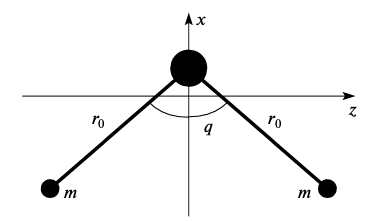
\includegraphics[width=0.4\textwidth]{../pictures/triatomic_fixed.png}
	\caption{Молекула $\ce{H2X}$ в подвижной системе отсчета.}
	\label{fig:triatomic}
\end{figure}

Выпишем координаты легких атомов в системе координат, связанной с центром масс.
\vverh
\begin{gather}
\left\{
\begin{aligned}
x_1 &= - r_0 \cos \lb \frac{q}{2} \rb \\
y_1 &= 0 \\
z_1 &= - r_0 \sin \lb \frac{q}{2} \rb 
\end{aligned}
\right. \quad \quad \quad
\left\{
\begin{aligned}
x_3 &= - r_0 \cos \lb \frac{q}{2} \rb \\
y_3 &= 0 \\
z_3 &= r_0 \sin \lb \frac{q}{2} \rb
\end{aligned}
\right.\notag
\end{gather}

Используя формулы, приведенные в предыдущей части, получим элементы матриц $\bba$, $\bbA$, $\bbI$, определяющих кинетическую энергию в форме Лагранжа в подвижной системе координат, учитывающей внутренние степени свободы. Размер матрицы $\bba$ равен $\dim \bba = s \times s$, где $s$ - количество внутренних степеней свободы, т.е. в данном случае матрица $\bba$ является числом: $\bba = \frac{I_0}{2}$, где $I_0 = m r_0^2$. Несложные преобразования показывают, что матрица $\bbA$ является нулевой. Тензор инерции рассматриваемой системы имеет диагональный вид, причем компоненты $I_{xx}$, $I_{zz}$ в сумме дают $I_{yy}$ (т.к. система плоская): $I_{xx} = 2 I_0 \sin^2 \lb \frac{q}{2} \rb$, $I_{yy} = 2I_0$, $I_{zz} = 2I_0 \cos^2 \lb \frac{q}{2} \rb$. Итак, кинетическая энергия 
в форме Лагранжа принимает следующий вид:
\vverh
\begin{gather}
T_\mathcal{L} = \frac{1}{2} \sum_i m_i \dot{\vec{R}}_i^2 + \vec{\Omega}^{\, \top} \sum_i m_i \left[ \vec{R}_i \times \dot{\vec{R}}_i \right] + \frac{1}{2} \vec{\Omega}^{\, \top} \bbI \ \vec{\Omega} = \frac{1}{2} \frac{I_0}{2} \dot{q}^2 + \frac{1}{2} \vec{\Omega}^{\, \top} \bbI \ \vec{\Omega}. \notag
\end{gather} 

Для перехода к кинетической энергии в форме Гамильтона применим формулы, полученные при помощи подхода Фробениуса к обращению блочных матриц. Т.к. $\bbA = \bbzero$: $\bbG_{11} = \bbI^{-1}$, $G_{12} = G_{21} = \bbzero$, $\bbG_{22} = \bba^{-1}$. Обращая матрицу тензора инерции и раскрывая матричное выражение в скалярное, получаем кинетическую энергию в Гамильтоновском представлении:
\vverh
\begin{gather}
T_\mathcal{H} = \frac{1}{2} \lb \frac{J_x^2}{I_{xx}} + \frac{J_y^2}{I_{yy}} + \frac{J_z^2}{I_{zz}} \rb + \frac{p^2}{I_0}, \notag
\end{gather}

В качестве потенциала, описывающего деформационное колебание, был взят потенциал Пешля-Теллера: $V = \frac{1}{2I_0} \lb \frac{V_{-}}{1 - \cos q} + \frac{V_{+}}{1 + \cos q} \rb$, где постоянные $V_{-}$, $V_{+}$ могут быть найдены исходя из равновесного значения угловой координаты $q_0$ и гармонической частоты деформационного колебания $\omega_0$:
\vverh
\begin{gather}
V_{\pm} = \frac{1}{4} I_0^2 \omega_0^2 (1 \pm \cos q_0 )^2. \notag
\end{gather}

Выбор потенциала обусловлен тем, что задача описания энергетического спектра квантового осциллятора с потенциалом этого типа допускает точное аналитическое решение:
\vverh
\begin{gather}
E_n = \frac{1}{I_0} \hbar^2 \left[ n + \frac{1}{2 \hbar} \lb \sqrt{V_{-}} + \sqrt{V_{+}} \rb \right] \times \left[ n + 1 + \frac{1}{2 \hbar} \lb \sqrt{V_{-}} + \sqrt{V_{+}} \rb \right], \quad n = 0, 1, 2, \dots \notag 
\end{gather}

Также отметим, что аналитическая зависимость эффективного потенциала $V_{eff.}$ (получение и смысл, которого будут объяснены в следующей части) от координаты $q$ аналогичен зависимости потенциала $V(q)$. Следовательно квантовую колебательную задачу с потенциалом $V_{eff.}$ можно рассматривать, считая компоненты вектора углового момента $J_\alpha, \ \alpha = (x, y, z)$ параметрами. То есть, спектр собственных значений будет описываться формулой того же вида:
\vverh
\begin{gather}
E_n = \frac{1}{I_0} \hbar^2 \left[ n + \frac{1}{2 \hbar} \left( \sqrt{V_{-} + J_x^2} + \sqrt{V_{+} + J_z^2} \right) \right] \times \left[ n + 1 + \frac{1}{2 \hbar} \left( \sqrt{V_{-} + J_x^2} + \sqrt{V_{+} + J_z^2} \right) \right], \notag \\ 
 \hspace{11cm} n = 0, 1, 2 \dots \notag
\end{gather}

Таким образом, каждый из уровней энергии $E_n$ осциллятора, существовавших в отсутствие вращения, при наличии вращения превращается в полосу, ширина которой определяется диапазоном возможных направлений вектора углового момента при его фиксированной длине (рисунок \eqref{fig:vib_levels}).

\begin{figure}[!ht]
  \centering
	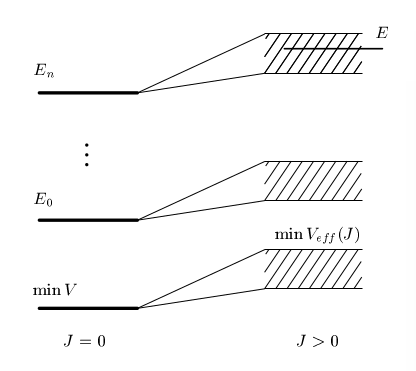
\includegraphics[width=0.5\textwidth]{../pictures/VibrationalLevels.png}
	\caption{Система колебательных уровней при отсутствии (слева) и при наличии (справа) вращения для одномерной задачи с потенциалом Пешля-Теллера.}
	\label{fig:vib_levels}
\end{figure}

\subsection{Концепция поверхности вращательной энергии.}

Концепция ПВЭ, впервые сформулированная Картером и Патерсоном [1], позволяет описать вращательную динамику молекул и связанную с ней природу квантовых вращательных спектров. ПВЭ представляет собой двумерную поверхность. Величина вращательной энергии откладывается в направлении вектора углового момента относительно молекулярно-фиксированной системы координат (при фиксированной длине вектора углового момента). Центросимметричность поверхности вращательной энергии является следствием наличия инверсии у вращательной задачи (изменение направления вращения системы приводит к обращению направления вектора углового момента, но сохраняет вращательную энергию). \\

Величина вращательной энергии определяется эффективным вращательным гамильтонианом, который может быть получен по следующей схеме. Рассмотрим компоненты вектора углового момента в качестве параметров в колебательно-вращательном гамильтониане $\mathcal{H} = \mathcal{H} (\vec{q}, \vec{p}, \vec{J})$. Определим равновесные значения обобщенных координат $\vec{q}_e = \vec{q}_e (\vec{J})$ и импульсов $\vec{p}_e = \vec{p}_e (\vec{J})$ как решения системы:
\begin{gather}
\left\{
\begin{aligned}
\lb \frac{\partial \mathcal{H}}{\partial \vec{q}} \rb_{\substack{\vec{q} = \vec{q}_e \\ \vec{p} = \vec{p}_e}} = \vec{0} \\
\lb \frac{\partial \mathcal{H}}{\partial \vec{p}} \rb_{\substack{\vec{q} = \vec{q}_e \\ \vec{p} = \vec{p}_e}} = \vec{0}
\end{aligned}
\right. \label{eff_ham}
\end{gather}

Эффективный вращательный гамильтониан получают заменяя обобщенные координаты $\vec{q}$ и сопряженные им импульсы $\vec{p}_e$ в колебательно-вращательном гамильтониане на их эффективные значения: $\mathcal{H}_r = \mathcal{H} (\vec{q}_e, \vec{p}_e, \vec{J})$.
Уравнения \eqref{eff_ham} могут быть рассмотрены с точки зрения модели ''мягкого тела''. При фиксированном направлении вектора углового момента внутренние координаты находятся в некотором новом равновесном состоянии, появившемся под действим центробежных сил. При этом внутримолекулярные колебания отсутствуют, и молекула вращается вокруг фиксированной в пространстве оси.
Между приближением Борна-Оппенгеймера и описанной процедурой можно провести определенные аналогии. В рамках первого приближения движения ядерной подсистемы принимают медленными по сравнениями с движениями электронной подсистемы, поэтому от суммарного гамильтониана системы переходят к электронному гамильтониану $\mathcal{H}_e$, параметрически зависящему от ядерных координат. В рамках описанной процедуры принимается, что самым медленным движением является вращение.
Второе векторное соотношение в системе \eqref{eff_ham} приводит к постоянству обобщенных координат: $\dot{\vec{q}} = 0$. Перепишем колебательно-вращательный гамильтониан в условиях $\vec{q} = \vec{q}_e$, $\vec{p} = \vec{p}_e$. Для этого получим выражение кинетической энергии в лагранжевых переменных $T_\mathcal{L} = T_\mathcal{L} (\vec{q}, \dot{\vec{q}} = \vec{0}, \vec{\Omega})$ и воспользуемся теоремой Донкина для перехода к гамильтоновым переменным:
\vverh
\begin{gather}
T_\mathcal{L}(\vec{q}, \dot{\vec{q}} = 0, \vec{\Omega}) = \frac{1}{2} \vec{\Omega}^{\, \top} \bbI \, \vec{\Omega} \quad \implies \quad T_\mathcal{H} = \frac{1}{2} \vec{J}^{\, \top} \bbI^{-1} \vec{J} \notag \\
\mathcal{H}(\vec{q}_e, \vec{p}_e, \vec{J}) = \frac{1}{2} \vec{J}^{\, \top} \bbI \, \vec{J} + V(\vec{q}_e) = V_{eff.} (\vec{q}_e, \vec{J}), \label{eff_ham2}
\end{gather}

\vlevo где $V_{eff.}$ -- эффективный потенциал. Соотношение \eqref{eff_ham2} позволяет получить зависимость $\vec{q}_e = \vec{q}_e (\vec{J})$, не решая систему \eqref{eff_ham}:
\begin{gather}
\lb \frac{\partial V_{eff.}}{\partial \vec{q}} \rb_{\vec{q} = \vec{q}_e} = \vec{0} \notag
\end{gather}

Т.к. построение поверхности вращательной энергии происходит при постоянном модуле вектора углового момента, то следует перейти к двум угловым переменным $\phi$, $\theta$, определяющим направление вектора углового момента. Таким образом уравнение ПВЭ принимает следующий вид: 
\vverh
\begin{gather}
E_r (\phi, \theta; J) = V_{eff.} (\vec{q}_e (\phi, \theta; J), \phi, \theta; J) \notag
\end{gather}

При анализе вращательной динамики сущесвенное значение имеют стационарные точки ПВЭ, их расположение на поверхности и их тип. Вследствие центросимметричности ПВЭ стационарные точки существуют в виде пар, эквивалентных относительно операции инверсии. Каждой паре симметрично расположенных точек соответствует одна ось, вокруг которой может вращаться вектор углового момнета. Устойчивость соответствующей оси зависит от типа стационарной точки: точки минимума и максимума порождают стабильные оси, а седловидные точки -- нестабильные. Положение стационарных точек может быть установлено при решении следующей системы уравнений:
\vverh
\begin{gather}
\left\{
\begin{aligned}
\frac{\partial E_r}{\partial \phi} = \frac{\partial V_{eff.}}{\partial \phi} + \frac{\partial V_{eff.}}{\partial \vec{q}_e} \frac{\partial \vec{q}_e}{\partial \phi} = 0 \\
\frac{\partial E_r}{\partial \theta} = \frac{\partial V_{eff.}}{\partial \theta} + \frac{\partial V_{eff.}}{\partial \vec{q}_e} \frac{\partial \vec{q}_e}{\partial \theta} = 0
\end{aligned}
\right. \notag
\end{gather}

Для определения типа стационарной точки необходимо исследовать знакоопределенность гессиана в окрестности исследуемой точки: 
\vverh
\begin{gather}
\mathds{H} = \begin{pmatrix}
\partial^2 E_r / \partial \phi^2 (\phi_s, \theta_s) & \partial^2 E_r / \partial \phi \partial \theta (\phi_s, \theta_s) \\
\partial^2 E_r / \partial \theta \partial \phi (\phi_s, \theta_s) & \partial^2 E_r / \partial \phi^2 (\phi_s, \theta_s)
\end{pmatrix}, \notag
\end{gather}
\vlevo где $(\phi_s, \theta_s)$ -- углы, определяющие положение рассматриваемой стационарной точки.

\subsection{Получение ПВЭ для трехатомных гидридов}

Построим эффективный гамильтониан исходя из колебательно-вращательного гамильтониана для модельной системы. 
\vverh
\begin{gather}
H(\vec{q}, \vec{p}, \vec{J}) = \frac{1}{2I_0} \left[ \frac{J_x^2 + V_{-}}{1-\cos q} + \frac{J_z^2 + V_{+}}{1 + \cos q} + \frac{J_y^2}{2} \right] + \frac{p^2}{I_0} \label{model_ham}
\end{gather}

Решение уравнений \eqref{eff_ham} дает нам выражения эффективных обобщенных координат и импульсов:
\begin{gather}
\left\{
\begin{aligned}
\cos q_e &= \frac{\sqrt{A_{+}} - \sqrt{A_{-}}}{\sqrt{A_{+}} + \sqrt{A_{-}}} \\
p_e &= 0,
\end{aligned}
\right.
\end{gather}

\vlevo где $A_{+} = J_z^2 + V_{+}$, $A_{-} = J_x^2 + V_{-}$. \\
Подставляем выражения эффективных координаты $q_e$ и импульса $p_e$ в гамильтониан \eqref{model_ham}, выполняя несложные алгебраические преобразования, приходим к следующему виду эффективного гамильтониана:
\vverh
\begin{gather}
H_r = \frac{1}{4I_0} \left[ \left( \sqrt{A_{+}} + \sqrt{A_{-}} \right)^2 + J_y^2 \right] \notag \\
E_r (\phi, \theta; J) = \frac{1}{4I_0} \left[ \left( \sqrt{V_{+} + J^2 \cos^2 \theta} + \sqrt{V_{-} + J^2 \cos^2 \phi \sin^2 \theta} \right)^2 + J^2 \sin^2 \phi \sin^2 \theta \right] \notag
\end{gather}

Построим несколько поверхностей вращательной энергии для молекулы $\ce{H2O}$ при разных значениях модуля вектора углового момента. 
\begin{figure}[H]
\begin{tabular}{|*7{c|}}  \hline
\rule[-2ex]{0pt}{6ex} & $\angle$ H-NonMe-H & $r_{e, NonMe-H}$, \AA & $\nu_1$, см$^{-1}$ & $\nu_2$, см$^{-1}$ & $\nu_3$, см$^{-1}$ & $\nu_{av.}$, см$^{-1}$  \\ \hline
\rule[-2ex]{0pt}{6ex} $\ce{H2O}$ & $104^\circ 31^{'}$ & $0,95718 \pm 0,0003$ & 3656,65 & 1594,78 & 3755,79 & 3706,22 \\ \hline
\rule[-2ex]{0pt}{6ex} $\ce{H2S}$ & $92^\circ 06^{'}$ & 1,3362 & 2614,56 & 1182,68 & 2625 & 2619,78 \\ \hline
\rule[-2ex]{0pt}{6ex} $\ce{H2Se}$ & $90^\circ 55^{'}$ & $1,460 \pm 0,03$ & 2344,50 & 1034,21 & 2357,80 & 2351,15 \\ \hline
\rule[-2ex]{0pt}{6ex} $\ce{H2Te}$ & $90^\circ 15^{'}$ & 1,658 & (2000) & 860,765 & (2000) & (2000) \\ \hline
\end{tabular}
\end{figure}

\begin{figure}[!ht]
  \centering
	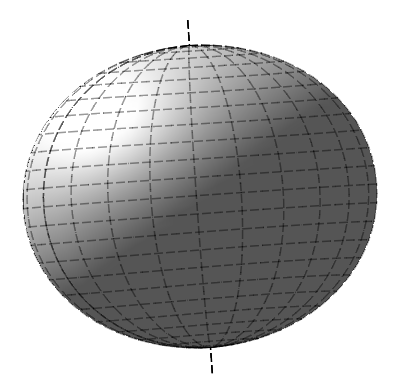
\includegraphics[width=0.25\textwidth]{../pictures/Rigid_RES_10.png}
	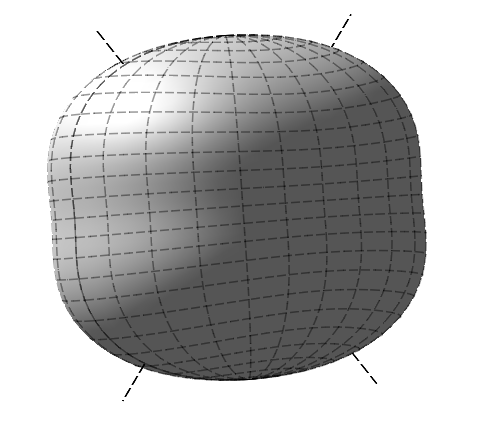
\includegraphics[width=0.3\textwidth]{../pictures/Rigid_RES_30.png}
	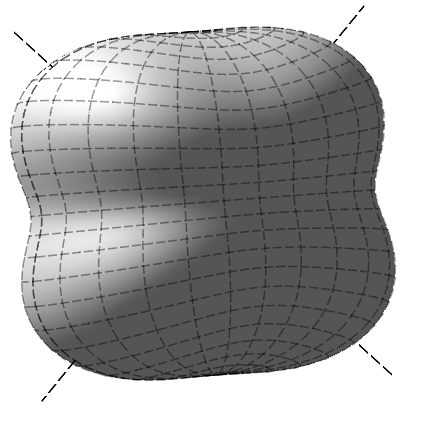
\includegraphics[width=0.3\textwidth]{../pictures/Rigid_RES_50.png}
	\caption{Перестройка поверхности вращательной энергии $\ce{H2O}$ при увеличении модуля вектора углового момента $J=10, 30, 50$.}
	\label{fig:triatomic}
\end{figure}

Несложно показать, что при малых значениях момента ПВЭ имеет две устойчивых оси вращения $Oz$ и $Oy$ и одну неустойчивую ось, проходящую через пару симметричных седловых точек. Таким образом, на ПВЭ имеется два типа прецессионных движений вектора углового момента -- вокруг оси $Oz$ (им соответствуют квантовые уровни в верхней части вращательного мультиплета) и вокруг оси $Oy$ (им соответствуют квантовые уровни в нижней части вращательного мультиплета). Анализ стационарных точек показывает, что перестройка ПВЭ наступает при достижении критического значения модуля углового момента:
\vverh
\begin{gather}
J_{cr.} = \sqrt{V_{-} - V_{+}} = I_0 \omega_0 \sqrt{|\cos q_0|} \label{critical_moment}
\end{gather}

При перестройки поверхности две точки максимума теряют свою устойчивость и становятся седловыми точками, в то время как возникают четыре новых точки максимума с координатами $(\theta_e, 0), (\theta_e, \pi), (\pi - \theta_e, 0), (\pi - \theta_e, \pi)$, где $\theta_e =\frac{1}{2} \arcsin \lb \frac{V_{-} - V_{+}}{J^2} \rb $. 

\section{Решение полной системы динамических уравнений}
Поверхность вращательной энергии является мощным инструментом, позволяющим на качественном уровне анализировать вращательную динамику молекулярной системы. Однако с ростом полной колебательно-вращательной энергии влияние колебательной подсистемы на вращение молекулы не может быть точно учтено в рамках эффективного гамильтониана. Следовательно необходимо решать полную систему динамических уравнений. При решении полной системы динамических уравнений необходимо надлежащим образом задавать начальные условия.

\subsection{Фазовые траектории одномерной модели.}

Система динамических уравнений, полученная из гамильтониана \eqref{model_ham}, выглядит следующим образом:
\vverh
\begin{gather}
\left\{
\begin{aligned}
\dot{\Phi} = \left( \frac{J_x}{I_0 ( 1 - \cos q)} \cos \Phi + \frac{J_y}{2I_0} \sin \Phi \right) &\ctg \Theta - \frac{J_z}{I_0 (1 + \cos q)} \\
\dot{\Theta} = \frac{J_x}{I_0 (1 - \cos q)} &\sin \Phi - \frac{J_y}{2I_0} \cos \Phi \\
\dot{q} &= 2	\frac{p}{I_0} \\
\dot{p} = - \frac{\sin q}{2I_0} \left( \frac{J_z^2}{(1 + \cos q)^2} - \frac{J_x^2}{(1 - \cos q)^2} \right) &- \frac{1}{2I_0} \left( \frac{V_{+} \sin q}{(1 + \cos q)^2} - \frac{V_{-} \sin q}{(1 - \cos q)^2} \right)
\end{aligned}
\right. \notag
\end{gather}

Решение представленной системы дифференциальных уравнений производилось при помощи математической платформы \textit{Maple 2015}. Возвращаясь к вопросу начальных условий, в качестве начального значения деформационного угла удобно использовать $q_0 = q_e$ (равновесного значения $q$ при фиксированном значении модуля вектора углового момента $J$). Переписывая выражение модельного гамильтониана \eqref{model_ham} через эффективный потенциал $V_{eff.}$, несложно получить начальное значение имупльса:
\vverh
\begin{gather}
E_n = \frac{p_0^2}{I_0} + V_{eff.} (q_0) \quad \implies \quad p_0 = \sqrt{I_0 \cdot \left( E_n - V_{eff.} (q_0) \right) } \notag
\end{gather}

Отметим, что положение $E_n$ внутри энергетической полосы (рисунок \eqref{vib_levels}) с номером $n$ определяется углами $\Theta_0$, $\Phi_0$, характеризующими направление вектора углового момента. 

\newpage

% modifying font of the appendix title
\appendix
\titleformat{\chapter}[display]
  {\normalfont\large\bfseries}% <- font for label "Appendix A", default \huge
  {\chaptertitlename\ \thechapter}
  {20pt}
  {\large}

\section{Про угловой момент..}
\begin{gather}
\left\{
\begin{aligned}
\vec{\Omega} = \frac{\partial \mathcal{H}}{\partial \vec{J}} \\ 
\vec{J} = \frac{\partial \mathcal{L}}{\partial \vec{\Omega}}
\end{aligned}
\right. \notag
\end{gather}

Доказательство первого соотношения представляет собой чисто техническую процедуру, так что опустим его. Продемонстрируем один из возможных путей доказательства второго соотношения:
\vverh
\begin{gather}
\vec{J} = \frac{\partial \mathcal{L}}{\partial \vec{\Omega}} = \bbA \dot{\vec{q}} + \bbI \, \vec{\Omega} \notag
\end{gather}

Для этого рассмотрим вектора углового момента в лабораторной системе координат и, используя ортогональную матрицу $\bbS$, выразим его через $\vec{\Omega}$ и $\left\{ \vec{R}_i \right\}$, представленные в подвижной системе координат:
\vverh
\begin{gather}
\vec{j} = \sum_{i=1}^{n} m_i \left[ \vec{r}_i \times \dot{\vec{r}}_i \right] \notag \\
\dot{\vec{r}}_i = \bbS^{-1} \lb \left[ \vec{\Omega} \times \vec{•}vec{R}_i \right] + \dot{\vec{R}}_i \rb \notag \\
\vec{j} = \sum_{i=1}^{n} m_i \left[ \vec{r}_i \times \bbS^{-1} \lb \left[ \vec{\Omega} \times \vec{R}_i \right] + \dot{\vec{R}}_i \rb \right] =
\bbS^{-1} \sum_i m_i \left[ \vec{R}_i \times \dot{\vec{R}}_i \right] + \bbS^{-1} \sum_i m_i \left[ \vec{R}_i \times \left[ \vec{\Omega} \times \vec{R}_i \right] \right] = \notag \\
= \bbS^{-1} \sum_i m_i \left[ \vec{R}_i \times \dot{\vec{R}}_i \right] + \bbS^{-1} \sum_i \lb R_i^2 \vec{\Omega} - \lb \vec{R}_i , \vec{\Omega} \rb \vec{R}_i \rb = \bbS^{-1} \bbA \dot{\vec{q}} + \bbI \, \vec{\Omega} \notag
\end{gather}

Умножая обе части на $\bbS$, приходим к искомому соотношению: 
\begin{gather}
\vec{J} = \bbS \vec{j} = \bbA \dot{\vec{q}} + \bbI \, \vec{\Omega} \notag 
\end{gather}

\section{Формулы Фробениуса}
\label{appendix:frobenius}
Рассмотрим интеграл некоторой функции $n$ переменных $\mf{x} = \lb x_1, \dots, x_n \rb$ по некоторой области $\Omega \subset \mathbb{R}^n$:
\vverh
\begin{gather}
I = \int\limits_{\Omega} f \lb \mf{x} \rb d \mf{x} \label{mint1} 
\end{gather}

Будем оценивать интеграл \eqref{mint1} задавая некоторое случайное распределение $M$ точек по $\Omega$ с плотностью вероятности $\rho(\mf{x})$:
\vverh
\begin{gather}
S^{\lb 1 \rb} = \frac{1}{M} \sum_{\mf{x}} \frac{f \lb \mf{x} \rb}{\rho \lb \mf{x} \rb} \, \longrightarrow I, \text{при} \, M \longrightarrow \infty. \notag
\end{gather}

Построенная оценка интеграла $S^{\lb 1 \rb}$ также является случайной величиной, ей дисперсия равна:
\vverh
\begin{gather}
\sigma^2 = \frac{1}{M} \left[ \int\limits_{\Omega} \frac{f^2 \lb \mf{x} \rb}{\rho \lb \mf{x} \rb} d \mf{x} - \lb \int\limits_{\Omega} f \lb \mf{x} \rb d \mf{x} \rb^2 \, \right] \notag
\end{gather}

При больших $M$ дисперсия аппроксимируется следующим выражением:
\vverh
\begin{gather}
\sigma^2 \simeq \frac{1}{M - 1} \lb S^{\lb 2 \rb} - \lb S^{\lb 1 \rb} \rb^2 \rb, \quad S^{\lb 2 \rb} = \frac{1}{M} \sum_{\mf{x}} \lb \frac{f \lb \mf{x} \rb}{\rho \lb \mf{x} \rb} \rb^2. \notag
\end{gather}

Среднеквадратичное отклонение $\sigma$ показывает насколько точно величина $S^{\lb 1 \rb}$ оценивает интеграл $I$ \eqref{mint1}. Существует несколько техник уменьшения СКО $\sigma$ при фиксированном $M$:
\begin{itemize}
\item Выборка по значимости (\textit{Importance sampling}). Идея метода заключается в том, что некоторые значения случайной величины имеют б\'{o}льшую значимость (вероятность) для оцениваемой функции чем другие. Если более значимые значения будут вносить больший вес в оценку интеграла, то дисперсия уменьшится. Несложно убедиться, что оптимальное распределение $\rho \lb \mf{x} \rb$  есть
\vverh
\begin{gather}
\rho \lb \mf{x} \rb = \ddfrac{| f(\mf{x}) |}{\int\limits_{\Omega} |f(\mf{x})| d \mf{x}} \notag
\end{gather} 
То есть, идея метода заключается в "концентрировании" плотности $\rho \lb \mf{x} \rb$ в тех областях $\Omega$, где $| f \lb \mf{x} \rb |$ максимально. 
\item Стратифицированная выборка (\textit{Stratified sampling}). Идея этого метода заключается в разбиении объема $\Omega$ на $N$ более маленьких объемов разных размеров. Интегрирование методом Монте-Карло выполняется в каждом из маленьких объемов с использованием $\frac{M}{N}$ точек. Изменяя относительный размер и расположение маленьких объемов, мы изменяем их вклад как в значение интеграла, так и в дисперсию. Общее значение дисперсии становится минимальным, когда вклад каждого объема одинаков и равен $\frac{\sigma^2}{N}$.  
\end{itemize} 

В чистом виде эти методики не применимы для general purpose алгоритмов интегрирования (т.е. для таких алгоритмов, которые не используют априорного знания о поведении подынтегральной функции), однако разработаны итеративные алгоритмы, позволяющие использовать информацию о подынтегральной функции, полученной в ходе одной итерации, для улучшения оценки в следующей. \cite{lepage1978, tsuda1973, haselgrove1961}


\section{Теорема Донкина}
\label{appendix:donkin}
\input{../appendices/appendix3.tex}

\end{document}